% Authors: Eric Sauvageat Please do not make changes to the preamble until after the solid line of
% %s.

\documentclass[12pt,a4paper,english,titlepage,twoside]{article}
\usepackage[report]{iaptitle}

\usepackage{hyphenat}
\usepackage{ragged2e}
\usepackage[utf8]{inputenc}
%\usepackage[pdftex,bookmarks=false,plainpages=false,pdfpagelabels]{hyperref}
%\usepackage[ansinew]{inputenc}
\usepackage{amsmath}                    
\usepackage{amsfonts}                   % fonts
\usepackage{amssymb}                    % symbols
\usepackage{fancyhdr}                   % fancy header
\usepackage{graphicx}                   % graphics
\usepackage{graphics}
\usepackage{textcomp}                   % graphics
\usepackage{color}
\usepackage[top=2.5cm,bottom=2.5cm,right=2.5cm,left=2.5cm]{geometry}
\usepackage{listings}
\usepackage{paralist}
\usepackage{comment}
%\usepackage[german,draft]{varioref}
\usepackage[english]{babel}
\usepackage{color}
%\usepackage{siunitx}
\usepackage{etoolbox}
\usepackage{float}
\usepackage{fancyref} % to use meta info in cross-referencing
\usepackage{hyperref}
\usepackage{mathtools}
\usepackage{enumerate}
\usepackage{media9}
%\usepackage[toc,page]{appendix}
\usepackage[titletoc]{appendix}
%\usepackage[]{subfloat}
\usepackage{todonotes}

\usepackage[nottoc]{tocbibind}
\usepackage{color, colortbl}

%\usepackage{subfigure}
\usepackage{indentfirst}
\usepackage{url}
\usepackage{subcaption}
\usepackage{gensymb}
\usepackage{color,soul}
\usepackage{lscape}
\usepackage{tabularx}
\usepackage{booktabs}
\usepackage{caption}
\graphicspath{{figs/}}

% Include any extra LaTeX packages required
\usepackage[square, numbers, comma, sort&compress]{natbib}  % Use the "Natbib" style for the references in the Bibliography
\usepackage{verbatim}  % Needed for the "comment" environment to make LaTeX comments
\usepackage{fancyhdr}
\usepackage[capitalise]{cleveref}
\usepackage[square,numbers]{natbib}
\bibliographystyle{apalike}% bibliography style
\setcitestyle{open={(},authoryear,close={)},}

%\RaggedRight

% These commands change the font. If you do not have Garamond on your computer, you will need to
%install it. \usepackage{garamondx}
\usepackage[T1]{fontenc}
\usepackage{amsmath, amsthm}
\usepackage{graphicx}
\usepackage{xcolor}

% This adjusts the underline to be in keeping with word processors.
\usepackage{soul}
\setlength{\parindent}{0pt}
\setlength{\parskip}{2em}

%%%%%%%%%%%%%%%%%%%%%%%%%%%%%%%%%%%%%%%%%%%%%%%%%

% Authors: Add additional packages and new commands here.  
% Limit your use of new commands and special formatting.

\title{User guide for the GROSOM calibration routine}
\author{Eric Sauvageat}
\date{December 2020}
\reportNr{...}

\begin{document}

% Makes the title and author information appear.
\maketitle

\section*{Summary}

This document contains a comprehensive description of the new GROSOM (GROMOS and SOMORA) calibration
routine. It should support new user of the calibration routine by describing the concept of the
routine, the functions and the underlying choices and methods applied during the calibration. It
could also help to include new instruments within the same calibration framework. 

This report also provides some examples of processing and highlights some of the changes introduced
with respect to the old calibration routines of GROMOS and SOMORA.

The complete reprocessing of the raw data from these two instruments will be the subject of a future
report and is not presented here. This future work will also contains a thorough identification of
suspicious calibrated data periods for both instruments.


\tableofcontents
\newpage
% Start the main part of the manuscript here. Comment out section headings if inappropriate to your
% discipline. If you add additional section or subsection headings, use an asterisk * to avoid
% numbering. 



\section{Introduction}

The GROund-based Millimeter-wave Ozone Spectrometer (GROMOS) and the Stratospheric Ozone Monitoring
Radiometer (SOMORA) are the only two Swiss radiometers measuring ozone profiles in the middle atmosphere (see Fig. \ref{fig:GROSOM}).

GROMOS is operated by the Institute of Applied Physics at the University of Berne while SOMORA is
operated by the Federal Office of Meteorology and Climatology MeteoSwiss in Payerne. 

Both instruments are part of the Network for the Detection of Atmospheric Composition Change
\href{http://www.ndaccdemo.org/}{NDACC} and operates continously since 1994 (GROMOS) and 2000 (SOMORA). 

long-term measurements very valuable for trends

Problems, see leonie

In November 2019, MCH and IAP decided 


\begin{figure}[h!]
  \centering
  \begin{subfigure}{.5\textwidth}
    \centering
    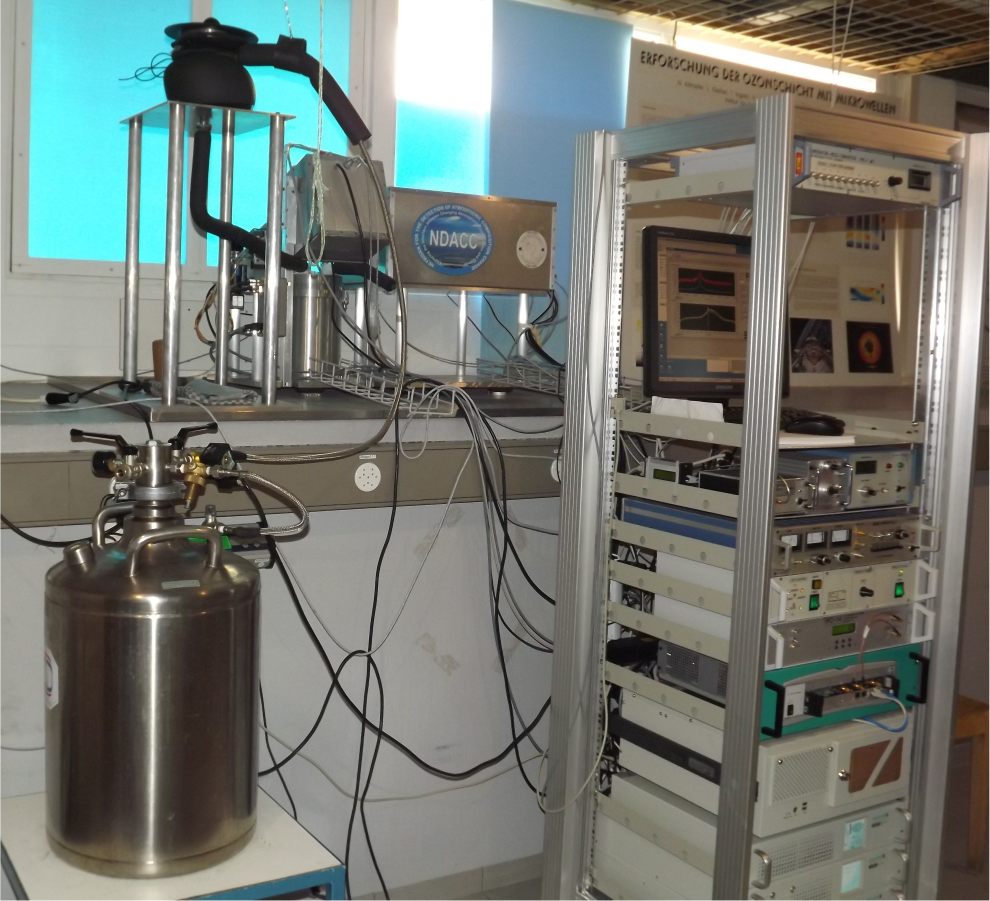
\includegraphics[height=60mm]{gromos_pics.png}
    \caption{GROMOS in Berne (IAP)}
    \label{fig:sub1}
  \end{subfigure}%
  \begin{subfigure}{.5\textwidth}
    \centering
    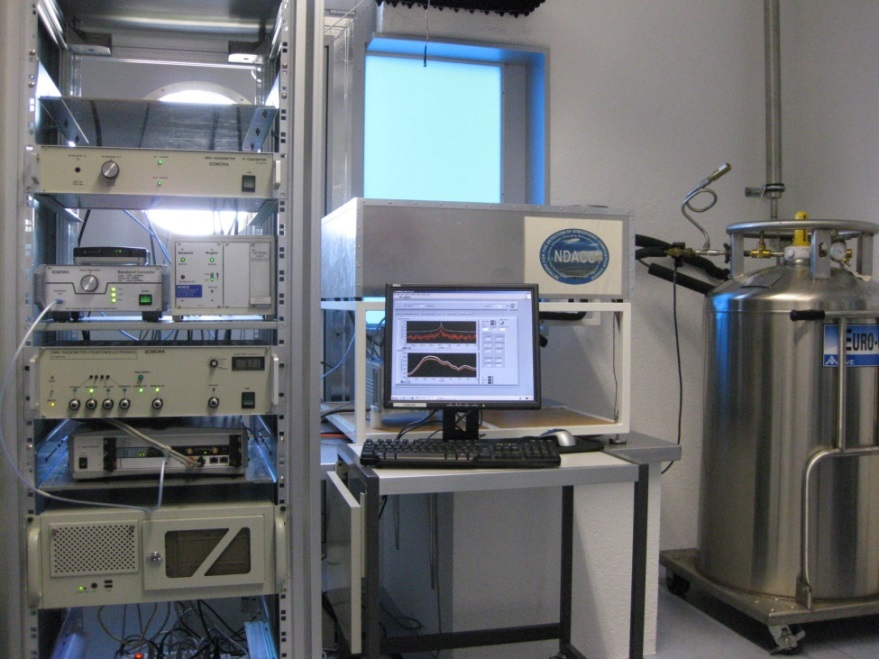
\includegraphics[height=60mm]{SOMORA_pic.jpg}
    \caption{SOMORA in Payerne (MeteoSwiss)}
    \label{fig:sub2}
  \end{subfigure}
  \caption{Pictures of the two radiometers}
  \label{fig:GROSOM}
  \end{figure}

\section{Using the routine}

\subsection{new subsection}

\section{Routine description}

\section{Comparison with the previous routine}

\section{Conclusion}


\end{document}
